% !TEXroot = ../thesis.tex

\chapter{Syntactic part} \label{sec:methodology}
Based on the Analytical part~\ref{sec:analytical} let us create  mathematical models to predict customer behavior which consist of
vendor, psychology and loyalty sub-models (see section~\ref {sec:submodels}) combined in Hidden markov model (HMM) to final prediction Customer behavior HMM.
We lead to get better results than predicting standard regression model methods (see section~\ref{sec:regression}) to predict customer behavior in e-commerce.
Finally, our approach will return future income for online store based on previous data with better aberration than linear or polynomial regression has.
Customer behavior HMM directly returns number of predicted orders than calculated to estimated income.
For successfully prediction will be used open data for store strength and customer satisfaction and some predefined and computed variables from store.

\section{Customer behavior HMM} \label{sec:submodels}
\begin{figure}[h!]
    \begin{center}
        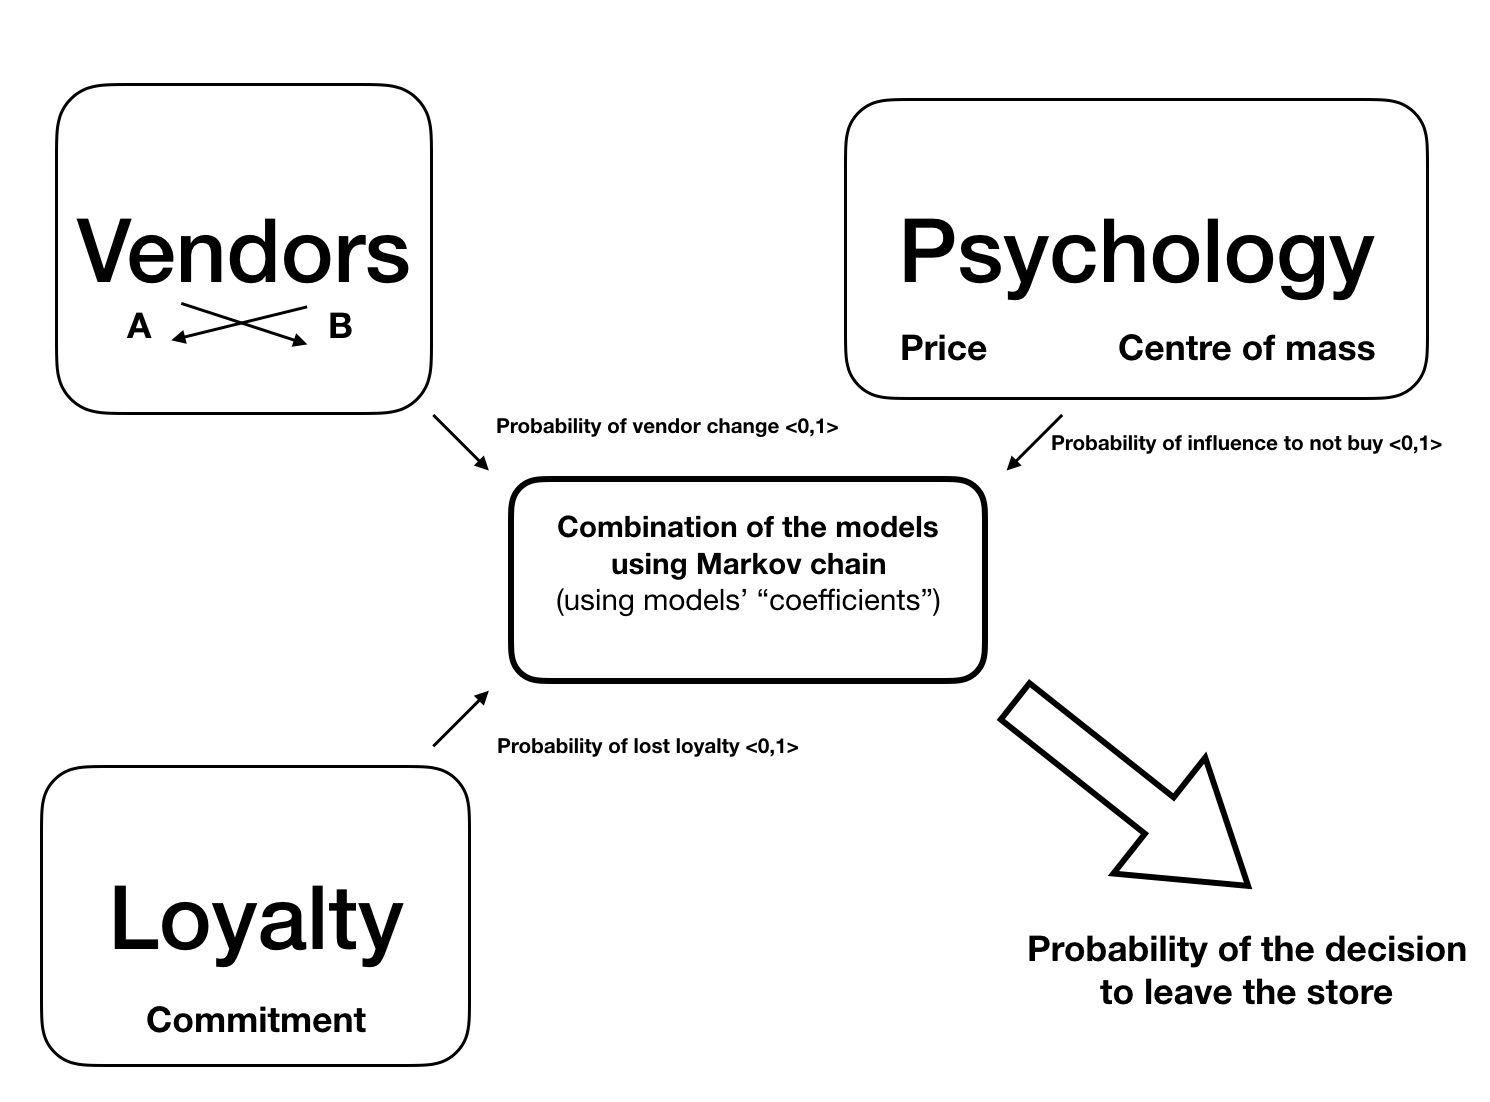
\includegraphics[width=100mm]{computation_schema.png}
    \end{center}
    \caption{Computation flow and interactions between models in Customer behavior HMM}
    \label{Model schema with interaction}
\end{figure}\\
Our model is based on Markov models (see section~\ref{markovmodel}) and consist of these three states: order, not finished order, no order decision.
Model simulate customer behavior during order process and trying to return the way with the most probability.
Then read the results by Viterbi algoritm and check if the order was made.
As inputs serves probabilities from predefined submodels used as transition matrix for HMM, number of customers in the predicted period,
probability matrix of initial states and average income per order by a previous period.
Our specific situation which is different from standard HMM is described on the figure~\ref{states} and tells that our states are not connected together as in HMM normally does.
This is caused by specific order process which are not directly connected each other.
In the first step model got predefined data from initial part (see section~\ref{sec:preprocessing}) and goes through the model according to the following steps:
\begin{enumerate}
    \item get probability from Vendor submodel (see section~\ref{subsec:model_vendors}),
    \item get probability from Psychology submodel (see section~\ref{subsec:model_psychology}),
    \item get probability from Loyalty submodel (see section~\ref{subsec:model_loyalty}),
    \item combine submodels data in Hidden Markov model (see section~\ref{subsec:combining_models}),
    \item read invisible states by Viterbi algoritm,
    \item check result matrix produced by viterbi and save the number of success orders,
    \item calculate prediction income.
\end{enumerate}\\
\begin{figure}[h!]
    \begin{center}
        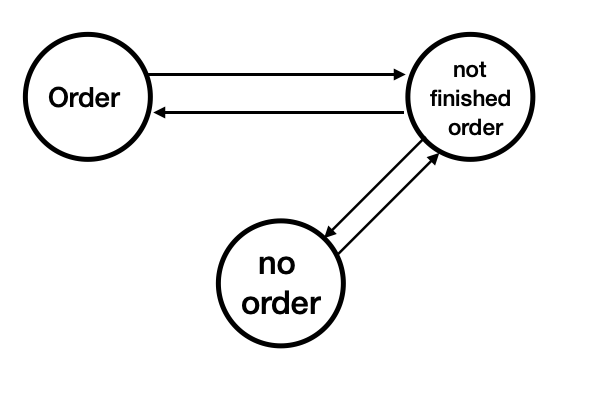
\includegraphics[width=80mm]{states.png}
    \end{center}
    \caption{Overview of states and their combinations}
    \label{states}
\end{figure}\\
On the figure~\ref{Model schema with interaction} the computation flow and interactions between models in Customer behavior HMM is presented.\\
\subsection{Vendors submodel} \label{subsec:model_vendors}
For simplification, we will take to account only a two vendors market share, without 100\% domination, because on a real
market is 100\% monopole unlikely to see and then we will be reflected only main competitor.
From that condition it is evident that for market to which dominate vendor it will return false positive results.
Our model is based on equations from Brands section~\ref{eq:10} and from those equations we will get probability of vendor
change from vendor $A$ to vendor $B$ and if the vendor $B$ will have more strength than vendor $A$ it will disrupt the
computation and customer will leave our store without completing buying process successfully.
Results of this computation wil be probability for each iteration of buying process simulation in an interval $<0,1>$.
Data for this model will come from open data provided by google.com, heureka.cz/heureka.sk and national governments.
That data will be combined with calculated price indexes downloaded from shopycrm.com tool.
\\
\begin{equation} \label{eq:13}
V_{xy} = \beta H(P_x-P_y) + \gamma H(Qx-Qy) + \delta H(Px-Py)H(Q_x - Q_y)
\end{equation}
\\
where $\beta, \gamma, \delta$ are non-negative~\ref{vendorCoeff}.
\\
\begin{itemize}
    \item $P$ is prices of vendors products
    \item $Q$ is a quality index of vendor
    \item $H$ is a Heaviside function which will be calculated by equation~\ref{eq:13}.
\end{itemize}\\
\\
\\
\begin{equation} \label{eq:14}
\begin{array}{l}
    H(s) = 1, s > 0 \\
    H (s) = 0, s \leq 0
\end{array}
\end{equation}
\\
\subsection{Psychology submodel} \label{subsec:model_psychology}
Psychology aspect is trying to simulate customer behavior in thee situation like a prices aspect, society influenced, mood aspect, actual needs
and so on.
In this model we will simplify only for price effect (see section~\ref{subsubsec:model_psychology_price}) and center of mass effect (see section~\ref{subsubsec:model_psychology_mass}).\\
\\
\textbf{Price aspect} \label{subsubsec:model_psychology_price} is described by equation~\ref{eq:15} and Center of mass is described by equation~\ref{eq:17}.\\
\\
\begin{equation} \label{eq:15}
\overset{-}{Q} = \frac{1}{n_p} \sum_{i=1}^{n_p} Q_i
\end{equation}
\\
\begin{itemize}
    \item $Q_i$ number of orders for product $i$ per day divide amount of orders per same day, prom interval $<0,1>$
    \item $n_p$ number of products in store
\end{itemize}
\\
\begin{equation} \label{eq:16}
\alpha_{ij} = \frac{C+max(Q_j, \overset{-}{Q})}{C+max(Q_i, \overset{-}{Q})}
\end{equation}
\\
Coefficient C is used to be $\alpha_{ij}$ always positive.
\textbf{Center of mass aspect} \label{subsubsec:model_psychology_mass} is applied as a part of sociology to our psyhology model.
Marketers use it for manipulating with customers in global way.
Like a black friday, Cyber monday etc., in that days stores manipulate with our psychology by discount prices.
\\
\begin{equation} \label{eq:17}
\overset{-}{P} = \frac{1}{n_p} \sum_{i=1}^{n_p} P_i
\end{equation}
\begin{itemize}
    \item $P_i$ is defined as product price minus retail recommend price divide average price
    \item $n_p$ number of products in store
\end{itemize}
\\
\begin{equation} \label{eq:18}
\beta_{ij} = \frac{C+max(P_j, \overset{-}{P})}{C+max(P_i, \overset{-}{P})}
\end{equation}
\\
This model returns final probability as count of $\alpha$ and $\beta$ probabilities for customer decision to make action from interval $<0,1>$.
\\
\subsection{Loyalty submodel} \label{subsec:model_loyalty}
This submodel is based on Luarn \& Lin research~\cite{luarn} and we changed theirs model for our needs.\\
\begin{equation} \label{eq:19}
L = \frac{R+Z}{Z}
\end{equation}
\\
\begin{enumerate}
    \item L ..... probability of whole loyalty model
    \item R ..... probability of separate loyalty model
    \item Z ..... probability of commitment model
\end{enumerate}
\\
As we see on figure~\ref{Loyalty scheme} Loyalty model consists of all three sub-models (Trust, Customer Satisfaction, Perceived value)
but commitment model consist of only Trust and Customer Satisfaction.
Weight coefficient $a,b,c,d,e$ were used to combine Trust, Customer satisfaction and Perceived value.\\
\begin{figure}[h!]
    \begin{center}
        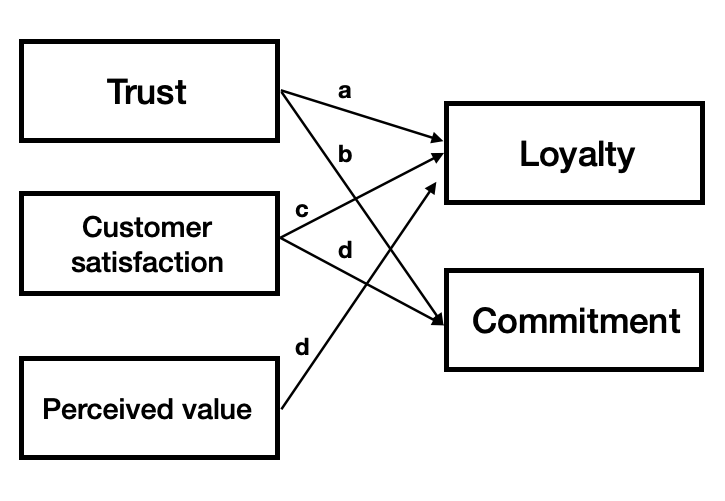
\includegraphics[width=100mm]{loyalty.png}
    \end{center}
    \caption{Computation flow for loyalty and commitment~\cite{luarn}}
    \label{Loyalty scheme}
\end{figure}\\
\\
\textbf{Trust}
\begin{equation} \label{eq:20}
T = \frac{1}{n} \sum_{i=1}^{n} O_i,
\end{equation}
\\
where $O_i$ number of orders divide number of visitors per day $i$.
\\
\\
\textbf{Customer satisfaction} are datasets get from open data per each day, individual satisfaction.
For simplified the situation we will use average satisfaction per whole store.
\textbf{Perceived value} (Se defined values in~\ref{perceived}) is subjective value, which depend on a strength of the store.
\subsubsection{Commitment and Loyalty} \label{subsubsec:model_loyalty_commitment}
\textbf{Commitment} is making the actual choice every day or other period basis to keep up with something e.g. a relationship, personal goal, a task, etc.
We would have to hold ourselves accountable to keep a commitment to something or someone.
Similarly, being loyal involves holding ourselves accountable as well.\\
Against of \textbf{Loyalty} which is usually seen as a character trait rather than a conscious decision.
This model return probability for customer decision to not leave the store from interval $<0,1>$.\\
\subsection{Combining submodels to decision process} \label{subsec:combining_models}
Appropriataly as a combination method was selected Hidden Markov Model (HMM).
All separates models return probabilities which was put together to square matrix used as input to HMM (see section~\ref{markovmodel}).
These probabilities will be combined with specific weights coefficients to always prevent positives results.
Let us created approach to store information from Customer behavior HMM about successfully order prediction.
In the same way the model is able to predict where the customer leaves the store, but this situation was not added to our prediction experiment and should be used in future updates.
Then based on that prediction data, calculation of future income for store were done.
Our designed model consists of three sub-models, which are partially dependent on each other.
Vendor,\ psychology and loyalty models we created for our prediction to simulate customer behavior.
Then partial results was combined into complex prediction mechanism, as you can see on figure~\ref{Model schema with interaction}.
\\
HMM in combination with Viterbi algorithm will be used to detect hidden states, which will be reflected in predefined weights for specific
industries to return data matrix with prediction.
Industry dependent on weights was set with Megaplay s.r.o employees, based on their data and experiences.
In a Hidden Markov Model (HMM), we have an invisible Markov chain (which we cannot observe), and each state
generates in random one out of $k$ observations, which are visible to us.
Let’s look at our situation.
Suppose we have the Markov Chain from above, with three states (order, not finished order and no order decision),
$P$ - the transition probability matrix and $q$ — the initial probabilities.
This is the invisible Markov Chain — suppose we are not with the customer and can not see the decision.
We can, however, see the results from the customer, and suppose there are two possible observations: order and no order decision.\\
With Megaplay s.r.o employees and heureka e-comerce tool calculation data were set probability wages vector for HMM function like:\\
$$ p_w = \left(\frac{1}{3} & \frac{1}{2} & \frac{1}{9}\right) $$
\\
This vector tells about probabilities for each hidden states described in own section~\ref{sec:submodels}
Vector have to be updated to square matrix which is used in Customer behavior HMM function like:\\
\begin{equation*}
    P_w =
    \begin{pmatrix}
        \frac{1}{3} & \frac{1}{2} & \frac{1}{9} \\
        \frac{1}{3} & \frac{1}{2} & \frac{1}{9} \\
        \frac{1}{3} & \frac{1}{2} & \frac{1}{9}
    \end{pmatrix}
\end{equation*}\\

\\
\section{Experiment} \label{experiment}
Let us prepare experiment to test our models.
We have prepared three models to create a prediction.
Data from section~\ref{sec:preprocessing} was used to predict the income for the year 2020.
We used Matlab to calculate linear regression analysis, polynomial regression analysis and prepare prediction application with Customer behavior HMM.
From each process we got real income for the year 2020, which were subsequently compared in Evaluation section~\ref{evaluation}.
Firstly we solved linear regression for model $f(x) = a(\sin(x-\pi))+b((x-10)^2)+c$.
The second one was polynomial model $f(x) = p_1x^4 + p_2x^3 + p_3x^2 + p_4x + p_5$.
At the last one we solved Customer behavior HHM as submodel combination in $P = (Y_n \in A|X_n = x_n)$ with probability matrix from section~\ref{subsec:combining_models}.
At a first glance we can see that the results from the models are different.
The first linear model with trigonometric function is not satisfying in real income results, but on the other hand was produced a very interesting result for trend prediction.
In contrast with polynomial model which has much better results in absolut income results, but much worse in trend prediction.\\
We compared prediction period and for each we calculate aberration against real store income from 2020.
Let us see our experiment in detail description and then see results in Evaluation section~\ref{evaluation} and Summary section~\ref{summary}.\\
\subsection{Preprocessing of input data} \label{sec:preprocessing}
The data comes from Megaplay s.r.o online stores and should have to be anonymized \footnote{Data anonymization is a type of information sanitization whose intent is privacy protection.
It is the process of either encrypting or removing personally identifiable information from data sets, so that
the people whom the data describe remain anonymous.} and pseudonymized \footnote{Pseudonymization is a data management
and de-identification procedure by which personally identifiable information fields within a data record are replaced
by one or more artificial identifiers, or pseudonyms.} to keep legal notice of~\cite{gdpr}.
Then we should utilize data to utilized inputs.
This prepared data will serve for baseline (Linear and polynomial models) and our prediction Customer behavior HMM.\\
\\
\textbf{Average day visitors for a predicted month}\\
This value was calculated from anonymize user data from Google Analytics tool used their prediction mechanism to get number of future users based on previous a number of visitors.\\
\\
\textbf{Perceived value for psychology model} \label{perceived}\\
This variable is needed for loyalty model~\ref{subsec:model_loyalty} and comes from an open e-commerce compare data provided by Heureka.cz/Heureka.sk internal tool.\\
\\
\textbf{Number of orders 2018 - 2019}\\
Number of orders we get from shopycrm.com tool used in Megaplay s.r.o to manage their business processes and also store all needed data.\\
\\
\textbf{Unique products sell}\\
This variable is used in Psychology model~\ref{subsec:model_psychology} for Price aspect calculation~\ref{eq:26}.\\
\\
\textbf{Customer satisfaction} \label{customerSat}\\
This value is provided by Heureka open data, and it's a calculated value from the all customer reviews of the store.\\
\\
\textbf{Margin}\\
The retail margin percentage measures the retail margin as a percentage of the retail price.
This measurement gives you a context for the retail margin.
For example, if you have a 5~€ retail margin on two different products, but one costs 150~€ and next one costs 10~€, the second product would have a much higher retail margin percentage.\\
\\
\textbf{Number of product order each day $Q_i$}\\
This is a calculated value from shopycrm.com about the number of product order for each one.
It's used in Psychology model~\ref{subsec:model_psychology}. \\
\\
\textbf{Quality index $Q_1$}\\
This is vendor quality index provided by Heureka open data.
This is a power/strength of the store.
Higher number means that for a customer is more difficult to leave the store and go to another online store.\\
\\
\textbf{Vendor coefficients $\beta, \gamma, \delta$} \label{vendorCoeff}\\
This three coefficients are used as weight for vendor model~\ref{subsec:model_vendors} and was set with cooperation with Megaplay s.r.o owner for their industry.
It represents the relation between vendor prices and vendor quality.\\
\\
\begin{table}[h!]
    \begin{center}
        \begin{tabular}{ | l | c |}
            \hline
            {\textbf{Variable name}} & \textbf{Result}\\
            \hline
            average day visitors for a predicted month $U_a$& 2357 \\
            perceived value for psychology model & 0.87 \\
            number of orders 2018 - 2019 $O_c$ & 26 530 \\
            Unique products sell $U_p$ & 11048\\
            Customer satisfaction & 90\%\\
            Margin & 0.27\\
            $Q_i$ & 4.12\\
            $Q_1$ & 0.94\\
            Vendor coefficients: & \\
            $\beta$ & 0.7\\
            $\gamma$ & 0.7\\
            $\delta$ & 0.85\\
            \hline
        \end{tabular}
    \end{center}
    \caption{Coefficient data from Megaplay s.r.o}
    \label{megaplay_data}
\end{table}
\\
\begin{table}[h!]
    \begin{center}
        \begin{tabular}{ | l | c |}
            \hline
            {\textbf{Variable name}} & \textbf{Equation}\\
            \hline
            number of visitors 1/2020 & $31 * U_a$\\
            average earn per order & $\sum Income / O_c$\\
            \overline{Q} & $1/U_p * (U_p/ O_c)$\\
            \overline{P} & $1/U_p * margin$\\
            trust & $1/O_c * O_c/U_a$\\
            \hline
        \end{tabular}
    \end{center}
    \caption{Calculated data from Megaplay s.r.o}
    \label{megaplay_data_equation}
\end{table}
\\
\subsection{Models for prediction} \label{sec:calculate_models}
As a baseline for our model will be used linear and polynomial fitting (see section~\ref{sec:regression}).
There are first two models which have to be solved.
The last one is our new Customer behavior HMM:\\
\begin{itemize}
    \item $f(x) = a(\sin(x-\pi))+b((x-10)^2)+c,$
    \item $f(x) = p_1x^4 + p_2x^3 + p_3x^2 + p_4x + p_5,$\\
    \item $P = \left(
    \begin{pmatrix}
        V_{xy} & V_{xy} & V_{xy} \\
        \alpha + \beta & \alpha + \beta & \alpha + \beta \\
        \frac{R + Z}{Z} & \frac{R + Z}{Z} & \frac{R + Z}{Z}
    \end{pmatrix}|
    \begin{pmatrix}
        l & m & k \\
        l & m & k \\
        l & m & k
    \end{pmatrix}
    \right)$,\\
    \\
    where $V_{xy}$ is vendor probability, $\alpha, \beta$ are partial results from psychology submodel, $R$ is partial
    loyalty and $Z$ is commitment probability. $l,m,k$ are a coefficients of initial states probabilities.
\end{itemize}\\
\\
\\
After solved the models the next parameters for models were identified:
\begin{table}[h!]
    \begin{center}
        \begin{tabular}{ | l | l | l |}
            \hline
            \textbf{linear model} & \textbf{polynomial model} & \textbf{Customer behavior HMM}\\
            \hline
            \makecell{$a =2.978.10^5$\\$b = 1687$\\$c = 1.753.10^6$} & \makecell{$p_1 = 225.1$\\$p_2 = -1.059.10^4$\\$p_3 =1.596.10^5$\\$p_4 = -8.205.10^5$\\$p_5 = 2.702.10^6$} & \makecell{$l = 1/2$\\$m = 1/3$\\$k = 1/9$}\\
            \hline
        \end{tabular}
    \end{center}
    \caption{Identified parameters for models}
    \label{parameters}
\end{table}\\
\textbf{Using random values for Customer behavior HMM}\\
In our model was randomly generated variables which was used to simulate situations from real store where the user can compare one store to another one in the different situation.
In other stores the situation should be better or worst to actual store.
To improve the results, it should be better to use data from real competitors from each trade, but it is not easy to obtain them.
This random variables are used as a simplification of that situation.\\
\\
All input data and models were prepared, so the prediction is have to be simulated.
Let us use data prepared in section~\ref{sec:preprocessing} and calculate prediction income from identified models.
\subsection{Compare results methodology} \label{subsec:matlab}
Finally we define the method to compare our models results.
Absolute number of income value prediction should not be important for the store owners because of that we calculated the aberration for each month
prediction and then we easily calculate quarterly and yearly results.
The sum of squared errors (SSE), defined by:
$$SSE = \sum^n_{i=1}w_i(y_i - \overline{y_i})^2,$$
between the fitting models and the used data serves as the fitting-criterion,
with values closer to $0$ indicating a smaller random error component of the model.
Also some other quality measures were evaluated, \textit{i.e.} the R-square from interval $[0,\ 1]$,
that indicates the proportion of variance satisfactory explained by the fitting-model (\textit{e.g.}  R-square $= 0.7325$ means
that the fit explains $73.25\%$ of the total variation in the data about the average);
R-square is defined as the ratio of the sum of squares of the regression (SSR) and the total sum of squares (SST).
SSR is defined as
$$SSR = \sum_{i=1}^nw_i(\overline{y_i} - \overline{y_i})^2.$$
SST is also called the sum of squares about the mean, and is defined as
$$SST = \sum_{i=1}^nw_i(y_i - \overline{y})^2,$$
where SST = SSR + SSE. Givenm these definition, R-square is expressed as
$$\frac{SSR}{SST} = 1 - \frac{SSE}{SST}.$$
The adjusted R-square statistic, with values smaller or equal to $1$, where values closer to $1$ indicate a better fit; the root mean squared error (RMSE):\\
$$RMSE = s = \sqrt{\frac{SSE}{v}}$$
with values closer to $0$ indicating a fit more useful for prediction~\cite{cftool}.
